\chapter{State of the Art}

\section{Isomorphisms Graph problem}

The Graph Isomorphism (GI) problem is very well known among computer scientists and mathematicians. It has been such a “star” target for algorithm designers that it was even referred to as a disease by researchers.~\cite{read1977graph}. GI belongs to the complexity class $\NP$ (cf.~\cref{def:NP}). However, it is still unknown whether a polynomial-time algorithm exists to solve it — in other words, it is not known whether GI belongs to the complexity class $\P$. Moreover, it is not known to be \NP{}-complete. GI was referred to as an ``open problem'' in the 1970s; a problem of which it was not known whether they were \NP{}-complete or in $\P$ (or neither)~\cite{garey2002computers}. Actually, its \NP{}-completeness is considered highly unlikely, as proving it \NP{}-complete would imply a collapse of the polynomial-time hierarchy (\PH) to its second level~\cite{goldreich1991proofs, schoning1988graph}—a result that would shake the foundations of computational complexity theory. This is especially problematic because it is widely conjectured that all levels of \PH{} are distinct and if \GI{} were \NP{}-complete, it would imply that all levels above the second would be equal to the second level.

For three decades, the fastest proven running time for the Graph Isomorphism problem was $e^{\mathcal{O}(\sqrt{n \log n})}$~\cite{babai1983computational}. But in 2016, it was shown that GI can be solved in quasi-polynomial time: $e^{\log(n)^{\mathcal{O}(1)}}$~\cite{babai2016graph}. Which makes one think even more that GI is only \NP{}-intermediate and not \NP{}-complete otherwise every problem in \NP{} could be solved in quasi-polynomial time.

Nonetheless, We already known some polynomial-time algorithms for GI for specific graph families.  These are often graphs with certain structural constraints, such as having a bounded Hadwiger number, a forbidden minor (see \cite{ponomarenko1988isomorphism} in Russian, as cited in \cite{mckay2014practical}), or an excluded topological subgraph~\cite{doi:10.1137/1.9781611973099.16}. Concrete examples of such graph classes include: graphs of bounded degree~\cite{luks1982isomorphism}, bounded tree-width~\cite{bodlaender1990polynomial}, and bounded eigenvalue multiplicities~\cite{babai1982isomorphism}, among others. The case of graphs with bounded genus was also addressed in earlier work~\cite{filotti1980polynomial}; however, the validity of the proposed polynomial-time algorithm was questioned later challenged~\cite{myrvold2011errors}.

For some of the graph classes mentioned, we can go even further. GI restricted to planar graphs and interval graphs can be solved in $\LOGSPACE$ (c.f \cref{def: logspace}), which represents a significant gain in terms of memory usage~\cite{darga2004exploiting, kobler2011interval}.

Unfortunately, most of these polynomial-time algorithms are theoretical and hard to implement in practice, with the exception of some well-structured families like trees~\cite{aho1974design}, planar graphs~\cite{10.1145/800119.803896}, and interval graphs~\cite{colbourn1981linear}.

Moreover, GI restricted to certains graphs do not change the difficulty of the problem; they are as hard as the general problem. Comme exemple de ces graphes, nous pouvons citer les graphes bipartis, chordal graphs, graphs of bounded degeneracy or even graphs of bounded expansion~\cite{grohe2012structural}.


To solve the Graph Isomorphism (GI) problem, three main types of algorithms must be considered~\cite{grohe2012structural}:

\begin{itemize}
    \item \textit{Graph theoretic algorithms}:
    Classical algorithms that exploit structural properties of specific graph classes.
    
    \item \textit{Group theoretic algorithms}:
    Based on computing generators for the automorphism group of a graph. These methods leverage group theoretic properties and have dominated GI research since the early 1980s.
    
    \item \textit{Combinatorial algorithms}:
    Simple and general purpose algorithms that do not rely on the specific structure of graph classes.
\end{itemize}

All combinatorial algorithms are based on the idea of \emph{colour refinement} (the 1-dimensional version of the Weisfeiler-Leman algorithm~\cite{kiefer2020power}), which aims to compute a \emph{stable colouring} of a graph.

\begin{algorithm}
\caption{Example of Colour Refinement Algorithm~\cite{grohe2012structural}}
\begin{algorithmic}[1]
\State \textbf{Initialisation:} Assign the same initial colour to all vertices.
\Repeat
    \State \textbf{Refinement Step:}
    \ForAll{pairs of vertices $v, w \in V$}
        \ForAll{colours $c$ in the current colouring}
            \If{the number of neighbours of $v$ of colour $c$ differs from that of $w$}
                \State Assign different colours to $v$ and $w$
            \EndIf
        \EndFor
    \EndFor
\Until{(the colouring is stable)}
\end{algorithmic}
\end{algorithm}


To use colour refinement as an isomorphism test, we apply it to the disjoint union of the input graphs $G$ and $G'$. The algorithm \emph{distinguishes} $G$ and $G'$ if there exists a colour $c$ in the stable colouring such that $G$ and $G'$ contain different numbers of vertices of colour $c$. Colour refinement \emph{identifies} a graph $G$ if it distinguishes $G$ from all non-isomorphic graphs; that is, no non-isomorphic graph shares the same stable colouring as $G$. However, if two graphs share the same stable partition, this is not a sufficient condition to prove that they are isomorphic; it is only a necessary one. Therefore, colour refinement does not fully solve the Graph Isomorphism problem, but rather provides a useful indication.

Colour refinement is not only used in the context of Graph Isomorphism; it also plays a role in reducing the cost of solving linear programs~\cite{grohe2014dimension}, as well as in computing graph kernels~\cite{shervashidze2011weisfeiler}.

Regarding the time complexity, for a graph $G$ with $n$ vertices and $m$ edges, a stable colouring can be computed in time $\mathcal{O}((n + m)\log n)$~\cite{cardon1982partitioning}, and has a lower bound of $\Omega((n + m)\log n)$ for the natural class of iterative partition refinement algorithms~\cite{berkholz2017tight}. This gives a tight bound of $\Theta((n + m)\log n)$ for such algorithms.


Now that the concept of colour refinement is well defined, we can turn to the types of combinatorial algorithms that build upon it:

\begin{itemize}
    \item \textit{Weisfeiler--Leman algorithm (or $k$-WL)}~\cite{kiefer2020power}: This is a generalization of the colour refinement algorithm. The principle remains largely the same, but instead of comparing individual nodes, the algorithm works on $k$-tuples of vertices. The central concept introduced is that of \textit{$i$-neighbours}. For $\vec{v}, \vec{w} \in V^k$ and for $i \in \{1, \dots, k\}$, the tuples $\vec{v}$ and $\vec{w}$ are said to be \textit{$i$-neighbours} if $v_j = w_j$ for all $j \neq i$.

    For a graph $G$ with $n$ vertices, the stable colouring computed by $k$-WL can be obtained in time $\mathcal{O}(n^k \log n)$.



\begin{algorithm}
\caption{$k$-dimensional Weisfeiler-Leman (k-WL) algorithm}
\begin{algorithmic}[1]
\Require Graph $G = (V, E)$, integer $k \geq 1$
\Ensure Stable colouring of $V^k$

\State \textbf{Initialization:}
\ForAll{tuples $\vec{v}, \vec{w} \in V^k$}
    \If{$\vec{v} \not\cong \vec{w}$} \Comment{No isomorphism between induced subgraphs}
        \State Assign different initial colours to $\vec{v}$ and $\vec{w}$
    \EndIf
\EndFor

\Repeat
    \State \textbf{Refinement step:}
    \ForAll{tuples $\vec{v}, \vec{w} \in V^k$}
        \For{$i = 1$ to $k$}
            \State Compare multisets of colours of $i$-neighbours of $\vec{v}$ and $\vec{w}$
            \If{they differ}
                \State Assign different colours to $\vec{v}$ and $\vec{w}$
            \EndIf
        \EndFor
    \EndFor
\Until{the colouring is stable}

\end{algorithmic}
\end{algorithm}

\item \textit{Individualisation-Refinement}: This approach consists of fixing vertices (individualisation) combined with the refinement of partitions of the vertex set. It was first introduced by Parris and Read~\cite{parris1969coding}, as cited in~\cite{mckay2014practical}). The first implementation of this technique appeared in \Naut. The key idea in \Naut is to construct a \textit{search tree}, where individualisation and refinement are applied recursively to guide the traversal. Once the search tree is fully constructed, a \textit{node invariant} function is applied in order to compute a \textit{canonical labelling} of the graph; a unique representation (or canonical form) of the graph. This canonical labelling is central to solving the graph isomorphism problem (GI): two graphs are isomorphic if and only if their canonical forms are identical.

\end{itemize}


Over time, several other GI solvers based on the individualisation-refinement Sparadigm have emerged:

\begin{itemize}
    \item \textit{Saucy}, introduced in 2004, has the same idea than \Naut but was designed to outperform it on sparse graphs~\cite{darga2004exploiting}. 
    
    \item A few years later, \textit{Bliss} was released. It also computes canonical forms but incorporates additional techniques that enhance performance on more complex graphs (\cite{junttila2011conflict}, as cited in~\cite{mckay2014practical}).
    
    \item \textit{Conauto}, introduced in 2009, has shown remarkable efficiency on random graphs and certain families of hard instances~\cite{lopez2011conauto}.
    
    \item Finally, \textit{Traces} was developed~\cite{piperno2008search}, a tool that can compete with \Naut in terms of performance on the Graph Isomorphism problem. Today, Traces and \Naut are tightly integrated and distributed together~\cite{mckay2014practical}.
\end{itemize}

\begin{figure}[H]
    \centering
    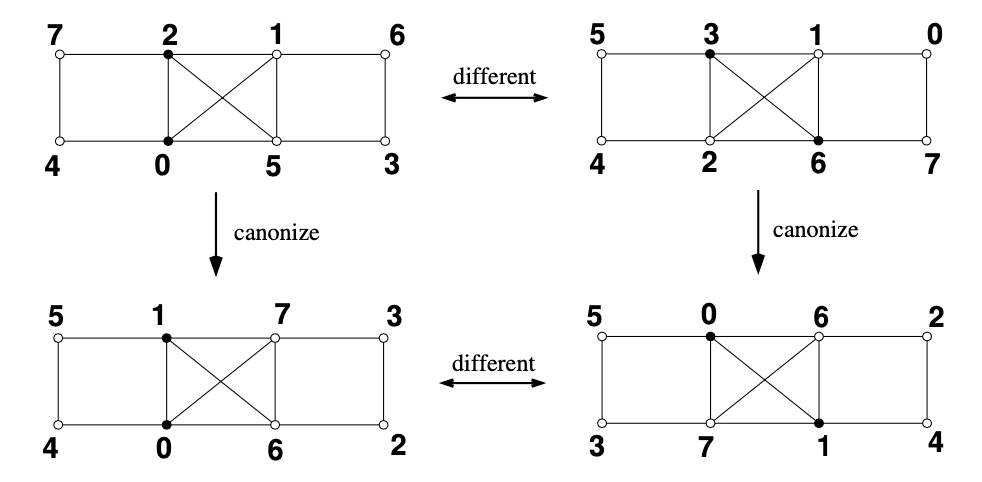
\includegraphics[width=0.8\linewidth]{imgs/pré-mémoire.png}
    \caption{Example of GI with canonical labelling from~\cite{mckay2024nug}}
    \label{fig: canonical labbeling}
\end{figure}


\medskip

Finally, An alternative approach to solving GI involves using linear programming. Given the adjacency matrices of two graphs $G$ and $H$, they are isomorphic if and only if there exists a permutation matrix $X$ such that $X^\top A X = B$.

This formulation can be relaxed using LP techniques, notably the Sherali--Adams hierarchy. In particular, level-$k$ Sherali--Adams relaxations offer a powerful framework that has been investigated for graph isomorphism testing~\cite{grohe2012structural}.



